% !TEX program = xelatex
% Edit the sample information and the files in chapters/ to begin your thesis.
\documentclass[12pt,fleqn]{report}

\usepackage[a4paper]{geometry}
\geometry{left=1.5in,right=0.85in,top=1in,bottom=1in,includeheadfoot}
\usepackage{fontspec}
\usepackage{xeCJK}
\setCJKmainfont{SimSun}
\setmainfont{Times New Roman}
\usepackage[shortcuts]{extdash}
\usepackage{etoolbox}
\makeatletter
\patchcmd{\chapter}{\if@openright\cleardoublepage\else\clearpage\fi}{}{}{}
\makeatother

\usepackage[utf8]{inputenc}
\usepackage[T1]{fontenc}
\usepackage{textcomp}
\usepackage{graphicx}
\graphicspath{{figures/}}
\usepackage{amsmath,amssymb,float}
\usepackage[labelsep=space]{caption}
% GB/T 7714 numerical citation and bibliography support.
\usepackage[square,sort,comma]{gbt7714}
\citestyle{numbers}

\setlength{\mathindent}{0pt}
\usepackage{indentfirst}
\setlength{\parindent}{0.75cm}
\setlength{\parskip}{0pt}

% Replace these sample values with the student's own information.
\newcommand{\thesistitle}{Brain Tumor Detection and Segmentation }
\newcommand{\studentname}{Mr John}
\newcommand{\studentid}{201735XX}

\usepackage{titlesec}
\titleformat{\chapter}[block]{\normalfont\normalsize}{\thechapter.}{0.5em}{}
\titlespacing*{\chapter}{0pt}{0pt}{6pt}
\titleformat{\section}[block]{\normalfont\normalsize\bfseries}{\thesection}{0.5em}{}
\titlespacing*{\section}{0pt}{6pt}{3pt}
\titleformat{\subsection}[block]{\normalfont\normalsize\bfseries}{\thesubsection}{0.5em}{}
\titlespacing*{\subsection}{0pt}{6pt}{3pt}

\usepackage{tocloft}
\usepackage{fancyhdr}
\pagestyle{fancy}
\fancyhf{}
\fancyhead[L]{\small 上海工程技术大学毕业设计（论文）}
\fancyhead[R]{\footnotesize \thesistitle}
\fancyfoot[C]{\thepage}
\renewcommand{\headrulewidth}{0.5pt}
\fancypagestyle{plain}{
  \fancyhf{}
  \fancyhead[L]{\small 上海工程技术大学毕业设计（论文）}
  \fancyhead[R]{\footnotesize \thesistitle}
  \fancyfoot[C]{\thepage}
  \renewcommand{\headrulewidth}{0.5pt}
}
\assignpagestyle{\chapter}{plain}

\renewcommand{\contentsname}{Table of Contents}

\begin{document}
\pagestyle{fancy}
\pagenumbering{arabic}
\setcounter{page}{1}
\tableofcontents
\clearpage

% The master project includes a Chinese abstract; keep it in this same position.
\begingroup
\titleformat{\chapter}[block]{\Large\normalsize\bfseries\centering}{}{0pt}{}
\chapter*{摘要}
\vspace{1em}
\addcontentsline{toc}{chapter}{摘要}
这是中文摘要示例。学生应在此处简要说明研究背景、研究方法、主要结果和结论，并替换为自己的论文内容。

\vspace{1em}
\noindent\textbf{关键词：} 示例论文，研究方法，模板
\endgroup
\clearpage

% The master project includes an English abstract; keep it in this same position.
\begingroup
\titleformat{\chapter}[block]{\Large\normalsize\bfseries\centering}{}{0pt}{}
\begin{center}
{\large\bfseries \thesistitle}\\[6pt]
{\small \studentname\ \studentid}
\end{center}
\vspace{0.8em}
\chapter*{ABSTRACT}
\vspace{1em}
\addcontentsline{toc}{chapter}{ABSTRACT}
\vspace{1em}
This is a sample abstract. Students should replace it with a concise description of their research background, methods, main findings, and conclusion.

\vspace{1em}
\textbf{Keywords:} sample thesis, research method, template
\endgroup
\vspace{2em}

% Keep the master project's title and student-information block before Chapter 1.
\clearpage
\begin{center}
{\bfseries \thesistitle}\\[6pt]
{\small \studentname\ \studentid}
\end{center}
\vspace{6pt}

% Thesis chapters: preserve the original master-project order.
% Chapter 1: replace the sample text while keeping the original chapter title and order.
\chapter{INTRODUCTION}

\section{Background}
This is a sample paragraph. Students should introduce the general research area and explain why the topic is important.

\section{Research Motivation}
This is a sample paragraph. Students should state the practical or academic problem that motivates the thesis.

\section{Thesis Overview}
This is a sample paragraph. Students should briefly explain the purpose, scope, and organization of the thesis.
% Chapter 2: use this file for a concise review of relevant literature.
\par
\chapter{RELATED WORK}

\section{Literature Overview}
This is a sample paragraph. Students should summarize the most relevant published work in their research area.

\section{Conceptual Framework}
This is a sample paragraph. Students should explain the theories, concepts, or technical approaches that guide the study.

\section{Research Gap}
This is a sample paragraph. Students should identify the gap addressed by the thesis and support the discussion with appropriate sources, for example \cite{lamport1994latex}.
% Chapter 3: describe the planned or completed research method here.
\par
\chapter{METHODOLOGY}

\section{Study Design}
This is a sample paragraph. Students should describe the overall design of the study and the rationale for the selected method.

\section{Data and Materials}
This is a sample paragraph. Students should identify the data, participants, instruments, materials, or software used in the study.

\noindent\textbf{GB/T 7714 numerical citations.} Cite a source in the text with \verb|\cite{key}|. For example, this template cites a journal article \cite{lecun2015deep}, a conference paper \cite{krizhevsky2012imagenet}, and a book \cite{lamport1994latex}. Add the corresponding entry to \texttt{ref.bib}; the existing GB/T 7714 bibliography style formats the reference list automatically.

% Citation guide adapted from the reference SUES template. Add or replace entries in ref.bib.
\begin{table}[htbp]
\centering
\small
\caption{GB/T 7714 reference-type and BibTeX entry guide}
\label{tab:gbt-reference-types}
\begin{tabular}{|p{2.2cm}|c|p{2.6cm}|p{5.2cm}|}
\hline
\textbf{Reference type} & \textbf{Code} & \textbf{BibTeX entry} & \textbf{Typical required fields} \\
\hline
Book & M & \texttt{@book} & author, title, publisher, year \\
\hline
Journal article & J & \texttt{@article} & author, title, journal, year, volume, number, pages \\
\hline
Conference paper & C & \texttt{@inproceedings} & author, title, booktitle, year, pages \\
\hline
Thesis or dissertation & D & \texttt{@mastersthesis} or \texttt{@phdthesis} & author, title, school, year \\
\hline
Technical report & R & \texttt{@techreport} & author, title, institution, year, number \\
\hline
Standard & S & \texttt{@misc} & authoring body, title, year, note or type \\
\hline
Online source & EB & \texttt{@misc} & author or organization, title, year, url, urldate \\
\hline
Other source & Z & \texttt{@misc} & author, title, year, note \\
\hline
\end{tabular}
\end{table}

\section{Analysis Procedure}
This is a sample paragraph. Students should explain how the data were processed and analysed. Equation~\eqref{eq:sample-mean} shows how to insert, label, and cite an equation in the text.

% Equation template: give every equation a unique label, then cite it with \eqref{...}.
\begin{equation}
\bar{x}=\frac{1}{n}\sum_{i=1}^{n}x_i
\label{eq:sample-mean}
\end{equation}

% Figure template: save image files in figures/, then replace the \input below with
% \includegraphics[width=0.8\textwidth]{your-figure-file.png}
% Keep a descriptive caption and a unique label; cite it as Figure~\ref{fig:sample-workflow}.
\begin{figure}[htbp]
  \centering
  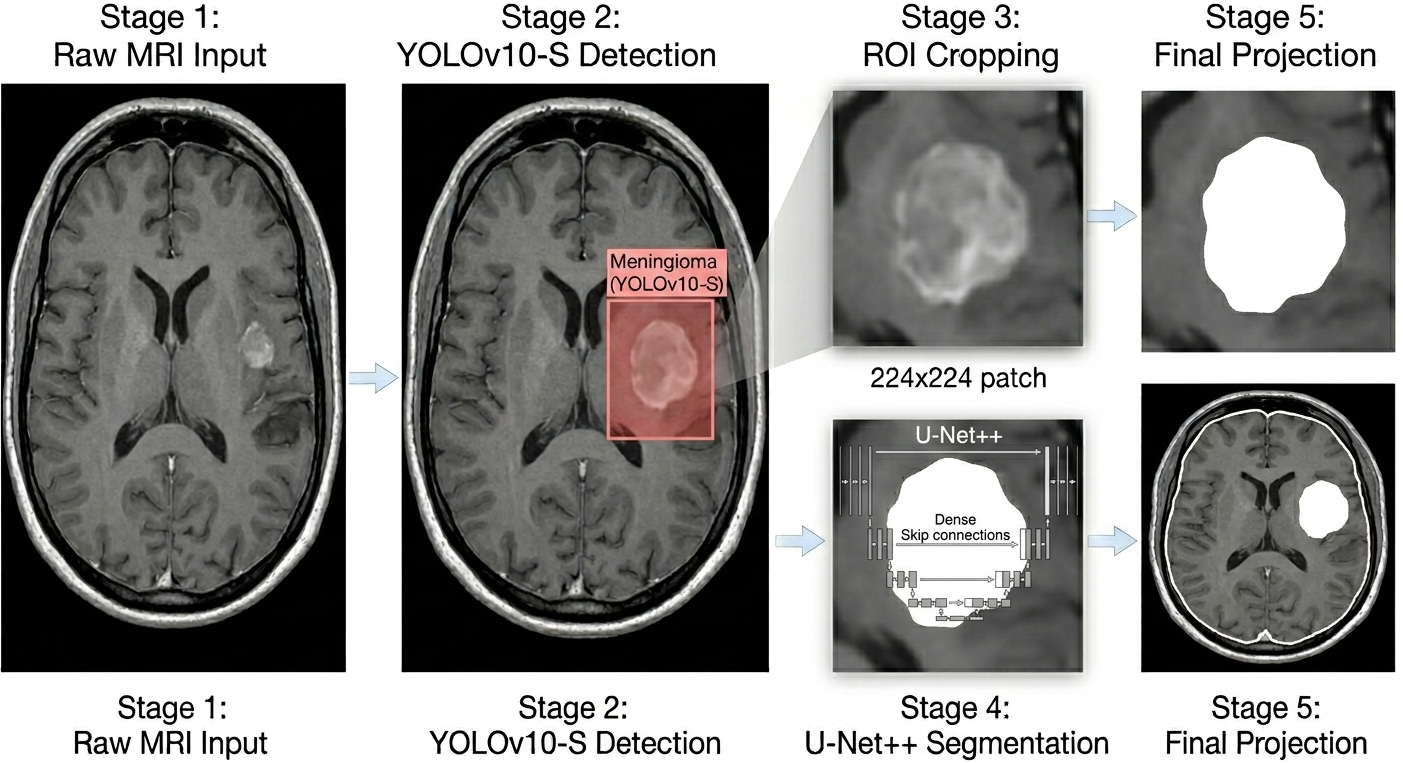
\includegraphics[width=0.85\textwidth]{sample-original-workflow.png}
  \caption{Sample workflow figure. Students may replace this example with their own image stored in the common \texttt{figures/} folder.}
  \label{fig:sample-workflow}
\end{figure}

Figure~\ref{fig:sample-workflow} demonstrates the required figure caption and cross-reference structure.

% Chapter 4: present results and interpret them in relation to the research questions.
\par
\chapter{EXPERIMENTS AND RESULT ANALYSIS}

\section{Experimental Setup}
This is a sample paragraph. Students should describe the test conditions, evaluation criteria, and settings used for their work.

\section{Sample Results}
This is a sample paragraph. Table~\ref{tab:sample-results} demonstrates a simple, reusable results table.

% Sample table structure adapted from the original thesis. Replace all entries.
\begin{table}[h]
\centering
\caption{Sample comparison metrics --- baseline versus proposed method.}
\label{tab:sample-results}
\begin{tabular}{|l|c|c|c|c|}
\hline
Configuration & Precision & Recall & F1-score & Overall Score \\
\hline
Baseline Method & 0.997 & 0.992 & 0.994 & 0.995 \\
Proposed Method & 0.990 & 0.977 & 0.983 & 0.987 \\
\hline
\end{tabular}
\end{table}

\section{Discussion}
This is a sample paragraph. Students should interpret the results, compare them with related work, and state any meaningful implications.
% Chapter 5: close the thesis without changing the original chapter title or order.
\par
\chapter{CONCLUSION AND FUTURE OUTLOOK}

\section{Summary}
This is a sample paragraph. Students should summarize the research objective, approach, and most important findings.

\section{Limitations}
This is a sample paragraph. Students should state the limitations of the study clearly and accurately.

\section{Future Directions}
This is a sample paragraph. Students should suggest realistic directions for future research or practical development.

% References retain the master project's GB/T 7714 bibliography style.
\newpage
\renewcommand\bibname{REFERENCES}
\bibliographystyle{gbt7714-2005-numerical_M}
\bibliography{ref}
\addcontentsline{toc}{chapter}{REFERENCES}

% The master project includes an acknowledgement; keep it after references.
\newpage
\begin{center}
{\large\bfseries ACKNOWLEDGEMENT}
\end{center}
\addcontentsline{toc}{chapter}{ACKNOWLEDGEMENT}
\vspace{1em}

This is a sample acknowledgement. Students may thank their supervisor, department, family, and others who supported their work. Replace this text with your own acknowledgement.

\vspace{2em}
\begin{flushright}
\studentid\quad \studentname
\end{flushright}

\end{document}
